\documentclass[12pt, titlepage]{article}
\usepackage{amsmath, mathtools}
\usepackage{amsfonts}
\usepackage{amssymb}
\usepackage{graphicx}
\usepackage{colortbl}
\usepackage{xr}
\usepackage{hyperref}
\usepackage{longtable}
\usepackage{xfrac}
\usepackage{tabularx}
\usepackage{float}
\usepackage{siunitx}
\usepackage{booktabs}
\usepackage{caption}
\usepackage{pdflscape}
\usepackage{afterpage}
\usepackage{amsmath} % for 'bmatrix' environment

\usepackage[round]{natbib}

\usepackage{amsmath}
\usepackage{booktabs}
\usepackage{tabularx}
\usepackage{hyperref}
\usepackage{siunitx}
\usepackage{csquotes}
\usepackage{graphicx}
\hypersetup{
    colorlinks,
    citecolor=blue,
    filecolor=black,
    linkcolor=red,
    urlcolor=blue
}
\usepackage[round]{natbib}

%% Comments

\usepackage{color}

\newif\ifcomments\commentstrue

\ifcomments
\newcommand{\authornote}[3]{\textcolor{#1}{[#3 ---#2]}}
\newcommand{\todo}[1]{\textcolor{red}{[TODO: #1]}}
\else
\newcommand{\authornote}[3]{}
\newcommand{\todo}[1]{}
\fi

\newcommand{\wss}[1]{\authornote{blue}{SS}{#1}} 
\newcommand{\plt}[1]{\authornote{magenta}{TPLT}{#1}} %For explanation of the template
\newcommand{\an}[1]{\authornote{cyan}{Author}{#1}}

%% Common Parts

\newcommand{\progname}{ProgName} % PUT YOUR PROGRAM NAME HERE %Every program
                                % should have a name


\renewcommand{\progname}{EEGSourceLocalizer} 
\begin{document}

\title{Test Report: \progname{} Software} 
\author{Leila Mousapour}
\date{\today}
	
\maketitle

\pagenumbering{roman}

\section{Revision History}

\begin{tabularx}{\textwidth}{p{3cm}p{2cm}X}
\toprule {\bf Date} & {\bf Version} & {\bf Notes}\\
\midrule
19 Dec, 2020 & 1.0 & First version of the VnV report\\
\bottomrule
\end{tabularx}

~\newpage

\section{Symbols, Abbreviations and Acronyms}


~\newline
\renewcommand{\arraystretch}{1.2}
\begin{tabular}{l l} 
\toprule		
\textbf{symbol} & \textbf{description}\\
\midrule 
T& Test\\
SRS & Software Requirements Specification\\
VnV & Verification and Validation\\
VnVR & Verification and Validation Report\\
MG& Module Guide\\
MIS& Module Interface Specification\\
EEGSourceLocalizer & Electroencephalogram Source Localization Software\\ 
EEG & Electroencephalogram \\
SL & Source Localization \\
\bottomrule
\end{tabular}\\

For completion, please see SRS Documentation at \url{https://github.com/LeilaMousapour/Brain-Computer-Interface-/ blob/master/docs/SRS/SRS.pdf}



\newpage

\tableofcontents

\listoftables %if appropriate

\listoffigures %if appropriate

\newpage

\pagenumbering{arabic}

This document is a report on the results of testing based on VnVP for \progname{} software.\ Detailed descriptions of the test cases can be found in the \href{https://github.com/LeilaMousapour/Brain-Computer-Interface-/tree/master/docs/VnVPlan}{VnV plan} documents.\ For each designed test, the data for the test case and the automated test script (if applicable) can be found in \url{https://github.com/LeilaMousapour/Brain-Computer-Interface-/tree/master/src} under test folder.

\section{Functional Requirements Evaluation}

\subsection{Static testing}

\subsubsection{Code walk-through}
\label{codewalk}

As mentioned in the design documents, this software is built on \href{https://www.fieldtriptoolbox.org}{Fieldtrip toolbox} which is an open source toolbox in MATLAB that offers source localization.\ The official tutorials of this toolbox are mainly designed and written for MEG data and are not directly applicable to EEG data.\ 
Thus, it is worth mentioning that the main problems with this software are due to the base scientific knowledge of the source localization problem in general and LCMV in particular and in these tests, the focus is not the pure programming challenges such as memory efficiency, style etc. .\ Therefore, the user has to take the challenge understanding every step of the SL problem, including the mathematical details of the forward and inverse problems profoundly in order to modifying all the steps for EEG data.\\

Even in the widely-used  \href{https://neuroimage.usc.edu/brainstorm/Introduction}{Brainstorm} application, which the user needs to interact with it through a GUI and it is more easier than coding up every step, the user need to have very good knowledge of the SL problem and the algorithm they are using in order to obtain meaningful results.\ Therefore, all the tests, including the static test of code walk-through are designed in a way to build confidence that mathematics of the problem is properly defined and implemented as different configuration, specifically for EEG data. Thus, this walk-through was designed in a more thorough way to go over the mathematical basics and checking the code accordingly.\\ 

Several sessions were held to walk the undergraduate student, Yar Mohammad Al Dabagh who working on the project through the code.\ The student and the developer both were assigned the bellow steps:

\begin{enumerate} 
	\item Read the LCMV base paper thoroughly and the necessary chapter of the source localization book \cite{veen_1997}
	\item Read and follow the Fieldtrip tutorial on \enquote{\href{https://www.fieldtriptoolbox.org/tutorial/beamformer/}{Localization of oscillatory sources}} in depth 
	\item The developer walked the student through every module of the software and explained how the implementation and different configurations matches the mathematics presented in the LCMV paper and why the chosen configurations are appropriate for EEG signal.
	\item The coding style and module design of the software was discussed.
	\item The quality of the comments was checked. 
	\item The simplicity of the main (control) module was checked.

\end{enumerate}

As a result of this test, several issues are revealed:

\begin{enumerate} 
	\item There was not enough understanding of the value that is calculated as \enquote{pow} in the output of the LCMC Fieldtrip function which will be plotted in the end. Thus, we could not interpret the result of the plots very well.
	\item The final source activity plots are basically plotting the -averaged- activity over the time period of the trial. It should be discussed and further looked into that how valid it is to look at and interpret the averaged activity of the sources as it is huge assumption.
	\item The source space of the sLORETA algorithm is not the whole brain and is only the cortical surface (a thin layer on the surface of the brain).
	
\end{enumerate}

\newpage
\subsection{Dynamic testing}

\subsubsection{test-input}
\label{test-input}
When the input EEG data is not meeting the condition (in-range amplitude and frequency), \progname{} will show an error. This test has been passed.

\subsubsection{test-rank}
\label{test-rank}
When the input EEG data is not full rank, \progname{} will show an error. This test has been passed.

\subsubsection{test-SimulatedEEG}
\label{test-SimulatedEEG}

In this test case, the input data (EEG) was manufactured based on the known solution (the location and strength of the sources).\ Recall, the sources are modeled as current dipoles. This test was done in 2 different configuration.\ First, the simplest case which is the EEG signal generated from one single source was tested.\ Next, to check the performance of the software in the presence of several sources with different strengths and orientations, the EEG signal generated from 3 separate dipoles was tested in the software.\\

In both tests, first the head model and the forward model (lead filed) were calculated based on the template ICBM 152 MRI. Then, using the ft\_dipolesimulation() function, by setting the configurations, the EEG signals were generated. Finally, a normal noise was with relative amplitude of 1/100000 was added to the signal. These EEG signals were plotted on the 2D electrode locations to confirm that the simulated EEG is as expected.\\

Additionally, this test was automated. After calculation of the sources time series and power, the maximum activity was found and the location of the source point corresponding tho the maximum activity was obtained. Afterwards, the distance between the distance between the location of the dipole that EEG is generated from and the location of the maximum activity in the software output is calculated and compared with the resolution of the head model grid (which is 1 cm as it is configured in the software code). If the distance is less than the grid resolution, the test will pass which in this case, it successfully passed. 

\begin{figure}[H]
\centering
  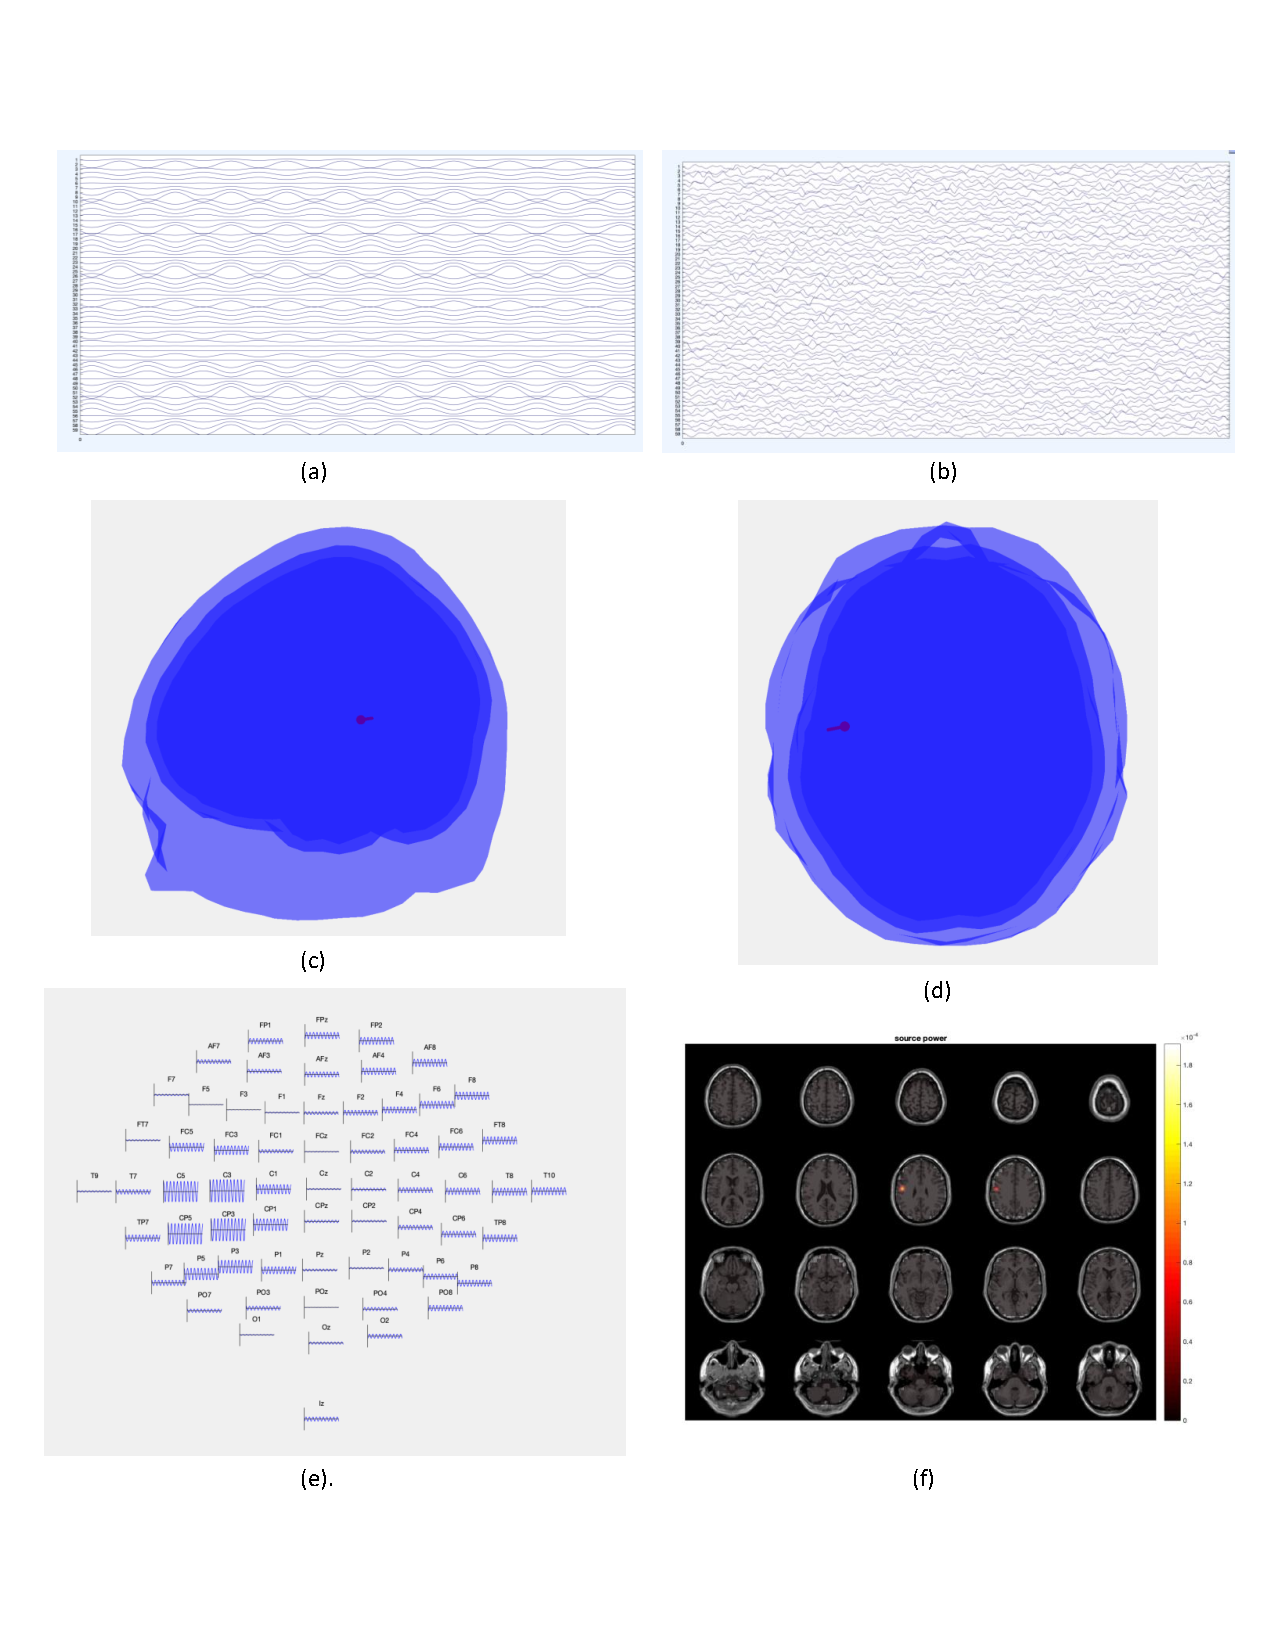
\includegraphics[scale=0.6]{1dipolsim_test.pdf}
  \caption{The result of EEG simulation test. (a) simulated EEG from one dipole on all channels. (b) simulated EEG plus noise. (c,d) the pre-defined location of the dipole that generates the EEG. (e) a 2D map of the signal at each channel. (f) the result of the software for localization of the simulated EEG  }
\label{Fig_1dip}
\end{figure}

\begin{figure}[H]
\centering
  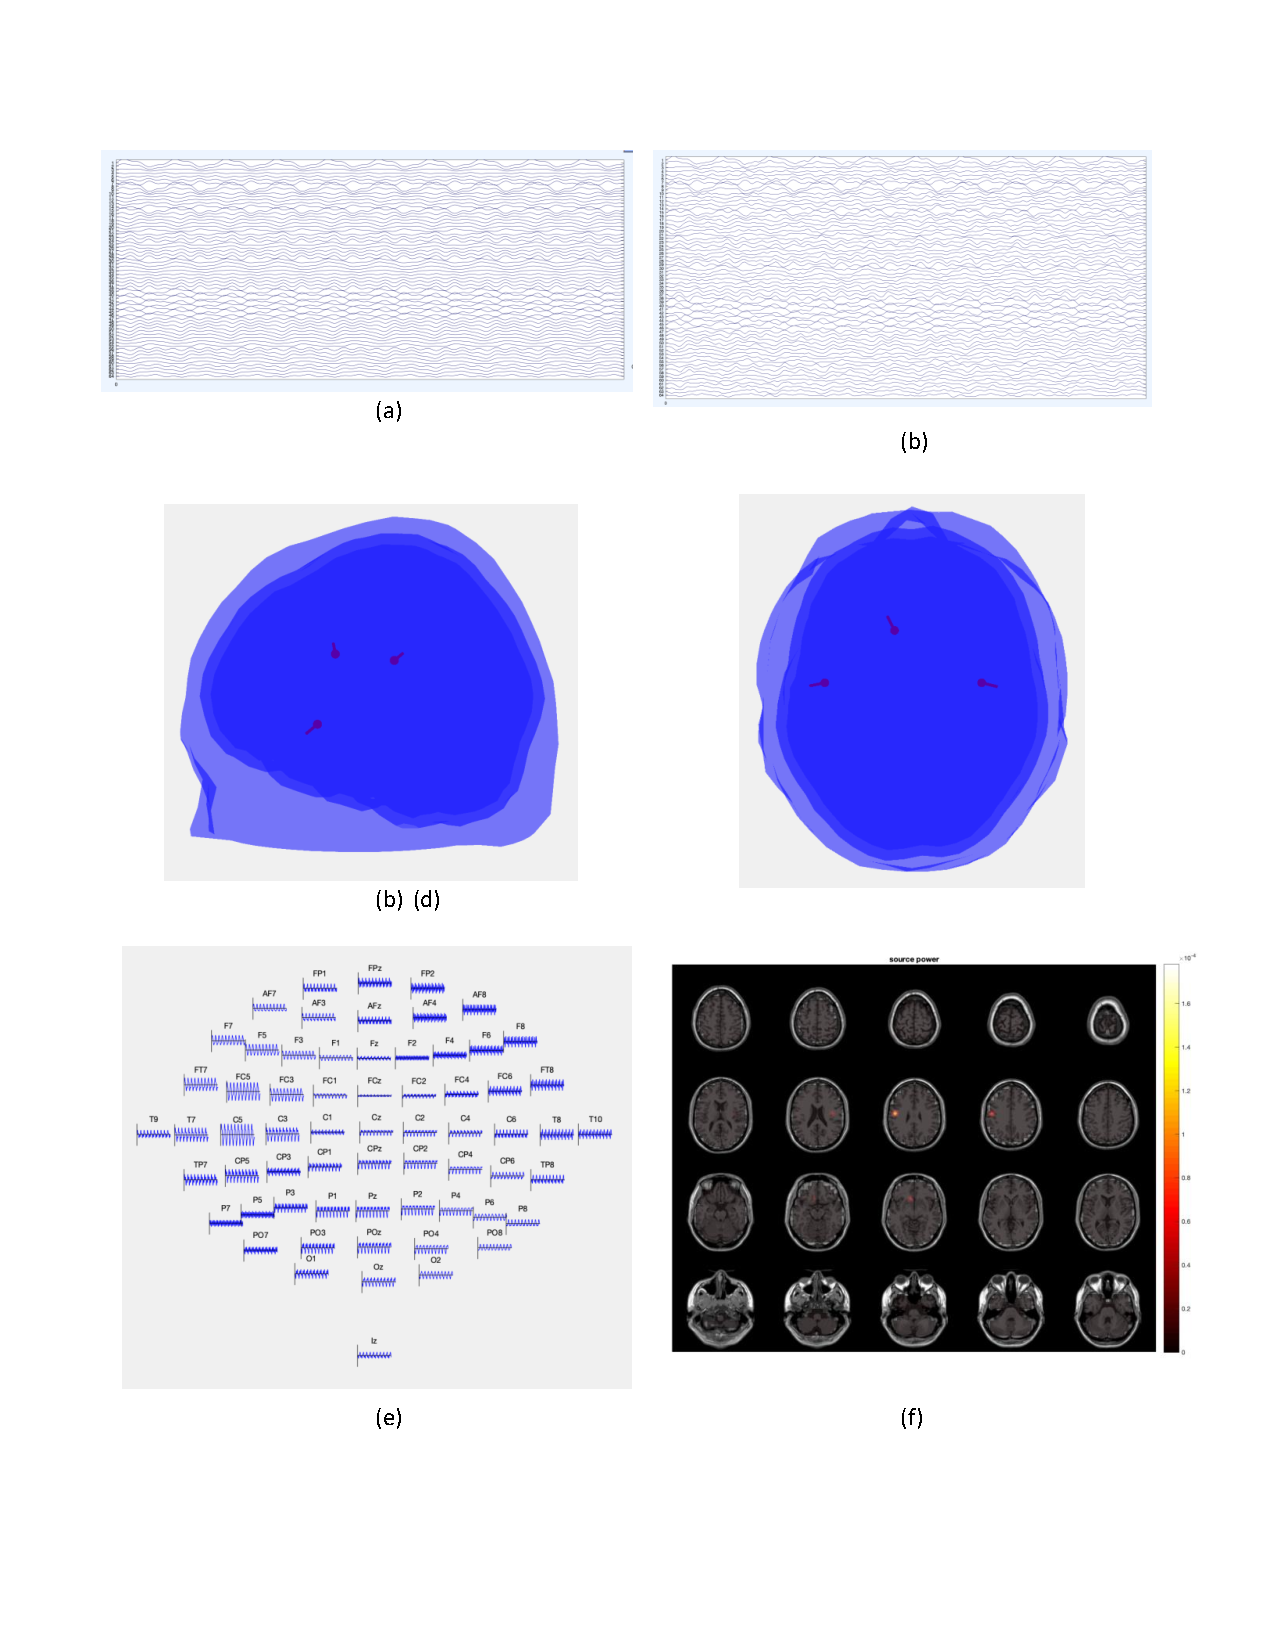
\includegraphics[scale=0.6]{3dipolsim_test.pdf}
  \caption{The result of EEG simulation test. (a) simulated EEG from three dipoles on all channels. (b) simulated EEG plus noise. (c,d) the pre-defined location of the dipole that generates the EEG. (e) a 2D map of the signal at each channel. (f) the result of the software for localization of the simulated EEG  }
\label{Fig_3dip}
\end{figure}

It is worth mentioning and recording that in the test case of 3 dipoles, when the frequency of the dipoles are not different, \progname{} is not able to localize 3 separate sources and it merges the sources. It is one of the shortcoming of the LCMV algorithms in general and it is due to the mathematics not the implementation or code.

\subsubsection{test-BrainstormPsudoOracle}
\label{test-BrainstormPsudoOracle}

Brainstorm application is a software for a variety of MEG/EEG signal processing including source localization. This application is controlled via a GUI and there are online tutorials on how to work with it. In this test, the \href{http://www.bbci.de/competition/iv/}{BCI iv dataset} is used. This dataset comprises of he data from 5 subjects which have performed 2 kind of moor imagery tasks over the period of 4 seconds. The goal is to locate the sources active in each of these 2 classes of motor imagery and classify them.\\

This test aimed to compare the numerical results of the sources time series extracted from Brainstorm (as a pseudo oracle) as the output result of the \progname{}. However, after learning how to work with Brainstorm and obtaining the result, I found out that this software uses \enquote{\href{https://openmeeg.github.io}{OpenMEEG}} to create the head model while I use \enquote{Dipoli} method for head model generation which makes the coordinate systems incompatible. Resolving this issue took plenty of time without any success so far. Therefore, in this test we only show the manual visual verification based on the source activity maps.\ As we can see based on the maps, the maps does not seem very similar.\ This problem should be look into further more.\\

\begin{figure}[H]
\centering
  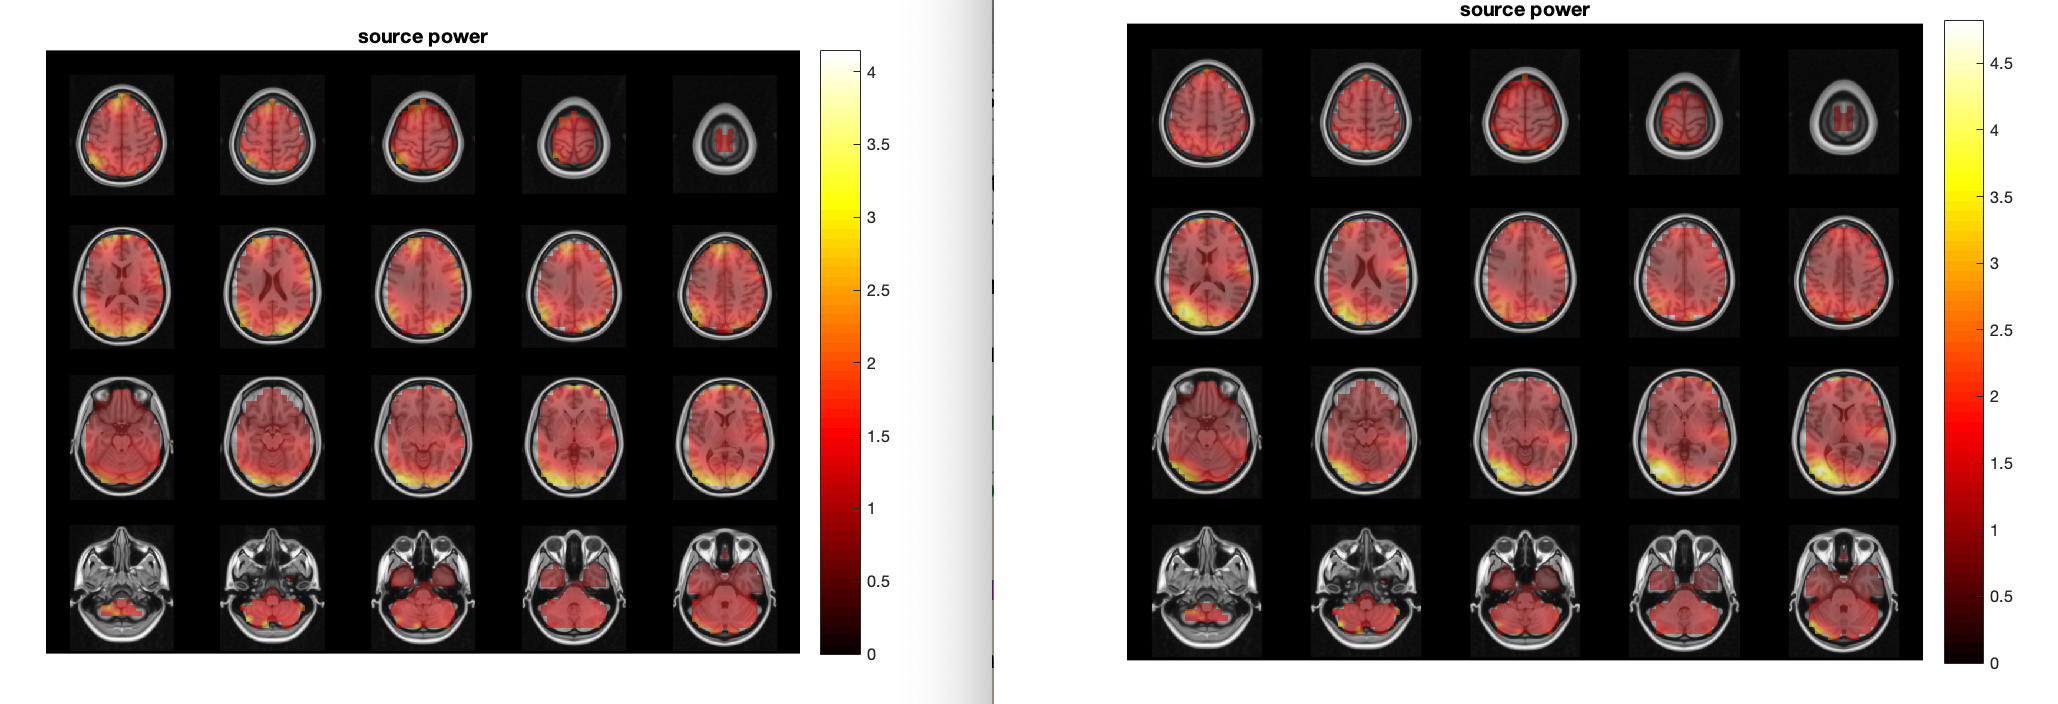
\includegraphics[scale=0.4]{bci_rightleft.png}
  \caption{The source power of right hand motor imagery is shown on the left and the source power of left hand motor imagery is shown on the right}
\label{Fig_bci}
\end{figure}

\begin{figure}[H]
\centering
  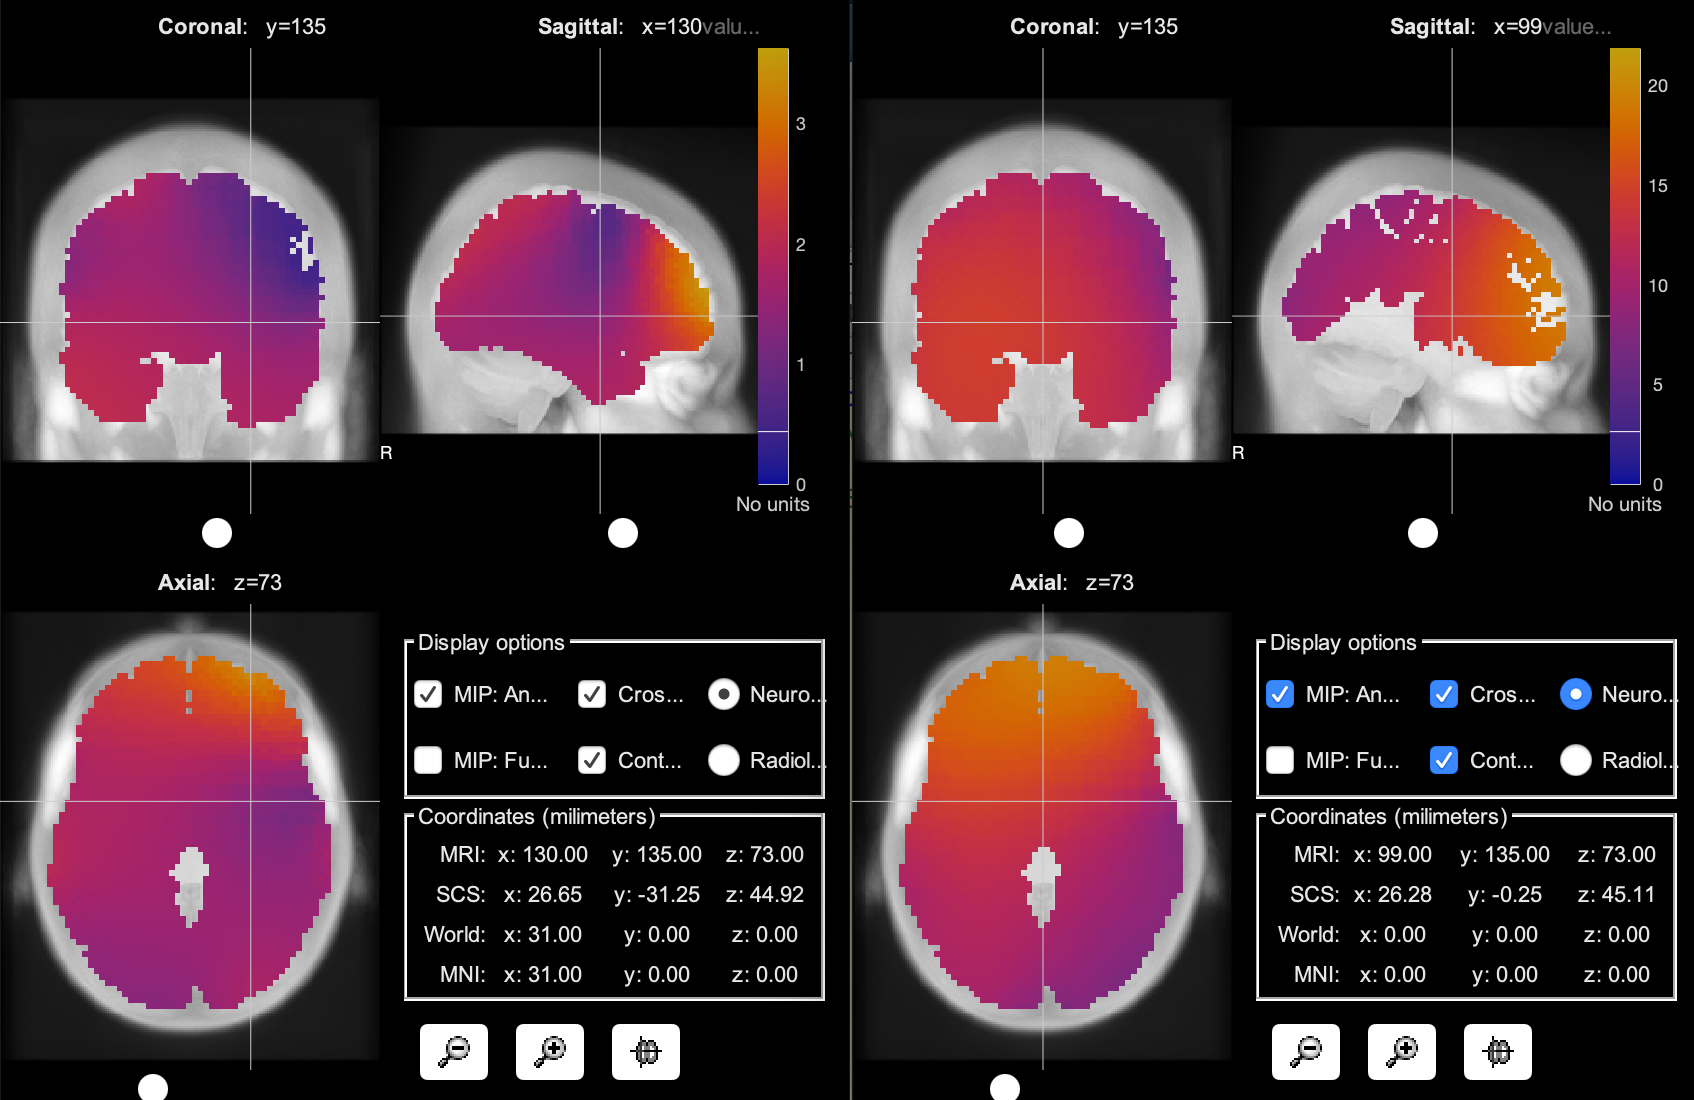
\includegraphics[scale=0.4]{bci_brainstorm.png}
  \caption{The source power of right hand motor imagery is shown on the left and the source power of left hand motor imagery is shown on the right}
\label{Fig_bci}
\end{figure}

\subsubsection{test-GroundTruthData}
\label{test-GroundTruthData}

As mentioned in the VnVP, \enquote{Simultaneous human intracerebral stimulation and HD-EEG, ground-truth for source localization methods} data set that comprises EEG recorded electrical activity originating from precisely known locations inside the brain of living humans \cite{Mikulan2020} can be used as a solid test case for any source localization procedure.\ Seven subjects participated in the study and a total of 61 sessions were obtained.\ Intracranial shafts were implanted using a robotic assistant and single-pulse biphasic currents lasting 0.5 ms were delivered at intensities ranging from 0.1 to 5 mA.\ EEG signals were recorded from 256 channels and sampled at 8000 Hz.\ The location of the intracranial electrodes was assessed registering the post-implant CT to the pre-implant MRI by means of the FLIRT software tool and these locations are provided in the dataset in MIN coordinate system.\ Contact positions were plotted on a flatmap of the MNI152 template by projecting each contact’s coordinates to the closest vertex of the brain surface reconstruction. A copy of the paper is included in the corresponding test folder\\

\begin{figure}[H]
\centering
  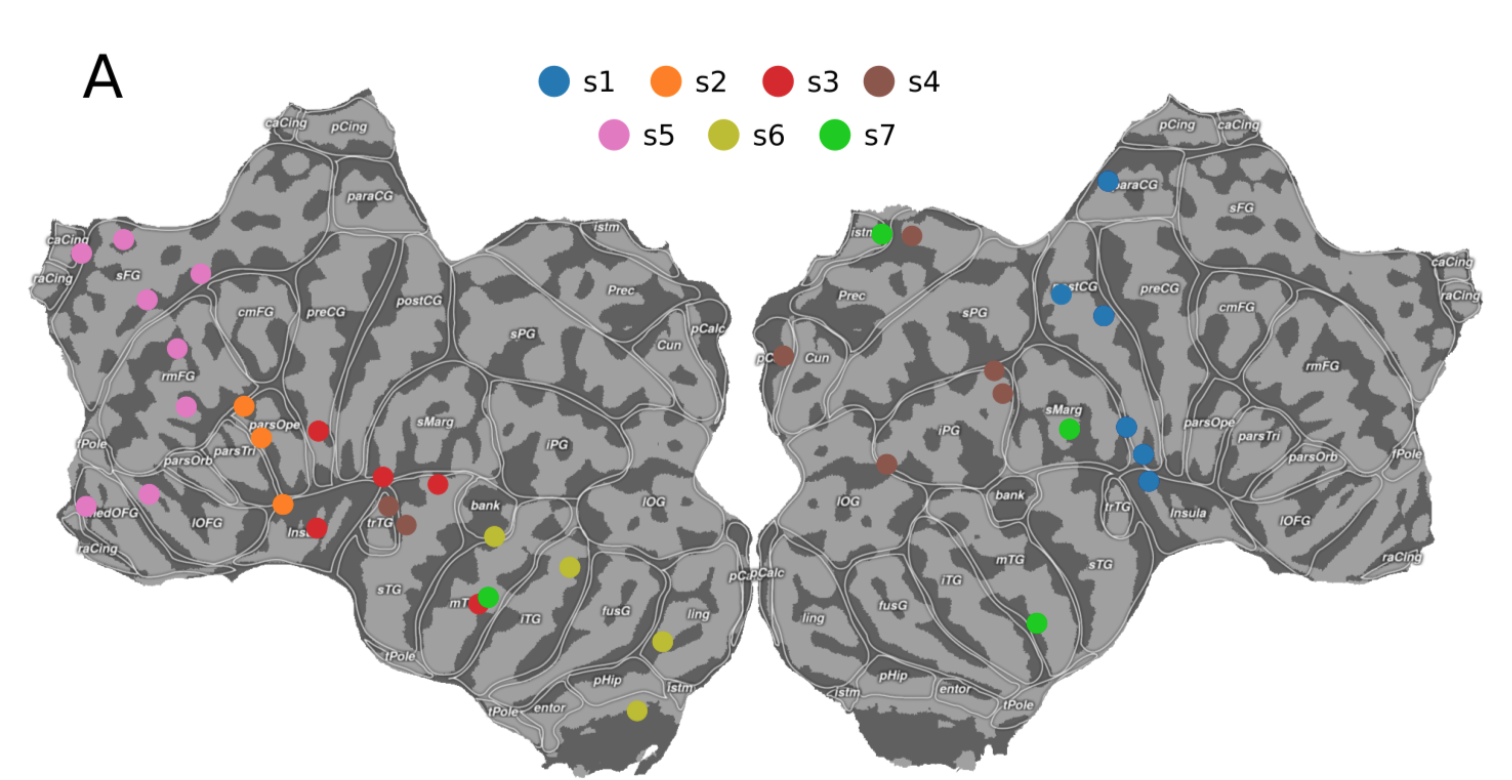
\includegraphics[scale=0.3]{GTflatmap.png}
  \caption{Flatmap of stimulation sites by subject \cite{Mikulan2020} }
\label{Fig_SolChar}
\end{figure}

In order to test this dataset, one run from each subject was chosen and the result is reported.\ The data in the dataset is provided in .npy format and has been read and transformed into .mat format by a python script. Also, the location of the implanted electrodes are provided. For each subject, the source localization was performed using the software.\ Recall that the activity of sources are estimated in time, thus it is important where in time we are looking at the source activity. After the presentation in the class (when I explained I could not get results from this data), the code walk-through brought out the point that -averaging- over time is a very big assumption. Also, a testing this data in the Brainstorm application, confirmed this point that we should look are the activity of the sources around the moment of the spike which is only 1ms and if we average over the whole 2500ms of the data, this activity will fade away. Therefore, in the automated test script in the \enquote{testGroundTruthData} folder, first the the time point in which the spike happens is located by finding the index of the maximum amplitude of the signal. Then, the activity of all the sources in that particular time point is obtained and the location of the source point with the maximum activity is found. The norm distance of this location and the actual location of the electrode is calculated and compared against the threshold of 30 mm. This threshold is chosen as based on the result in the paper, localization error varied between 1~20mm for the 3 algorithms they tested the data on. Thus, this software would pass the test if it can localize the source by the penalty of 10mm.\\

 The result of this test on one run of every subject is reported in table \ref{GTresult} and compared with the result of the paper. Also, for demonstration purposes, the source activity plot and the actual and estimated location of the source inside the head model is included for one of the subjects (subject5-run01).\ As we can see, \progname{} has the ability of locating the source within an acceptable error range for subjects 1 and 5 and for other subjects it is a relatively big error which shows the need for more parameter tuning in the \progname{}.\ It is important to note that the min localization error reported in the paper is the result of extensive hyperparameter tuning.\ A total of 4800 solutions were calculated for each session and then the best solution across all montages and parameter’s configurations was computed and reported in the paper. \\
 
 \begin{table}
 \caption{The result of the ground truth dataset  mm}
 \centering
    \begin{tabular}{| l | l | l | l | l |}
    \hline
    Sbj & Run & Software error & Paper min error  & Pass\\ \hline
    sbj1 & 01 &15.39 & ~5 &  Pass\\ \hline
    sbj2 & 01 & 81.33 & ~6 & Not Pass\\ \hline
    sbj3 & 01 & 37.92 & ~6 & Not Pass\\ \hline
    sbj4 & 01 & 53.98 & ~4 & Not Pass\\ \hline
    sbj5 & 01 &18.48& ~6 & Pass\\ \hline
    sbj6 & 01 & 42.10 & ~5 & Not Pass\\ \hline    
    sbj7 & 01 & 66.30 & ~6 & Not Pass\\ \hline
    \end{tabular}
\label{GTresult}
\end{table}

\begin{figure}[H]
\centering
  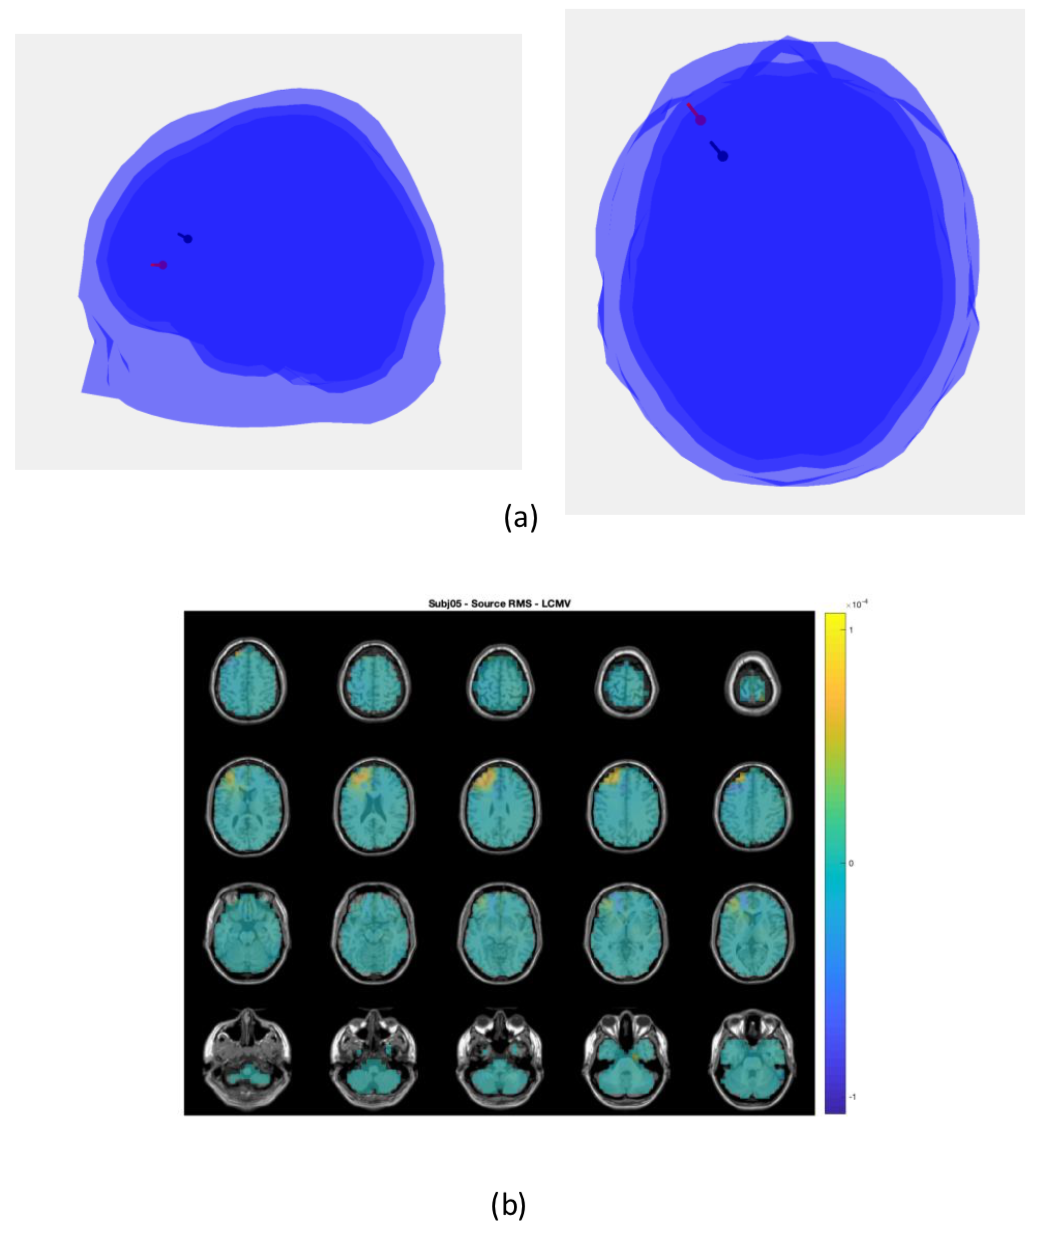
\includegraphics[scale=0.5]{GTsbj5.png}
  \caption{(a) The estimated dipole location is shown in black and the actual location of the implanted electrode is shown in blue. (b) The activity of the sources at the moment of the spike }
\label{Fig_GTsbj5}
\end{figure}



It is very much worth mention that during this test I learnt a very important information about the way the ft\_sourceanalysis() produces the results.\ This important point is that the results of source localization are in the in NM or CTF space which are 2 coordinate systems.\ However, I have always been comparing the locations of the sources with locations in the MNI coordinations system which is a huge mistake.\ Automation of this test, which required comparing the locations of the implanted intracranial electrodes with the result the software produces made me realize this longterm mistake!\\

%sbj5-run07: channel X'2_3, 0.3 mA
\section{Nonfunctional Requirements Evaluation}

\subsection{Accuracy}

As explained in the VnVP and as you could see from the testings, due to the nature of the problem, testing the accuracy is very hard for an arbitrary EEG data as we do not know the true solution to compare our results with. The ground truth dataset is a way of testing the accuracy of the software which the results are reported in section \ref{test-GroundTruthData}.
\section{Unit Testing}

\section{Changes Due to Testing}

Each of the tests mentioned in previous sections revealed different errors or lack of understanding. As a summary, these changes were made to the software:

Additionally, \progname{} is far from perfect and these modifications and test should be applied on this software in the near future:

\begin{itemize}
\item Automate the code to find the best setting and configuration of LCMV appropriate to the data
\item The result of the LCMV algorithm should be similar to other SL algorithms and should be tested against them.
\item sLORETA algorithm must be added to the software as stated in the SRS.
\end{itemize}


\section{Trace to Requirements}

\begin{table}[h!]
	\centering
	\begin{tabular}{|c|c|c|c|c|c|c|c|c|c|c|c|c|c|c|c|c|c|c|c|c|}
		\hline        
		& R1 & R2 & R3 & R4 & R5 & NR1 \\
		\hline
		test-input        &X & & & & & \\ \hline
		test-rank        & &X & & & &  \\ \hline
		test-SimulatedEEG        & & &X & X& & \\ \hline
		test-BrainstormPsudoOracle        & & & &X & X& X \\ \hline
		test-GroundTruthData   & & & &X & X& X \\ \hline
	\end{tabular}
\caption{Traceability Matrix Showing the Connections Between Tests and Functional and Nonfunctional System Requirements}
\label{Table:A_trace}
\end{table}


\section{Trace to Modules}

\begin{table}[h]
    \begin{tabular}{|l|l|l|l|l|l|l|l|l|l|}
        \hline
         Test& M2 &M3 & M4 & M5 & M6 & M7 & M8 \\ \hline
       code walkthrough \ref{codewalk} & X &X  & X & X & X &X &X\\ \hline
       test-input \ref{test-input} & X &  &  &  &  & & \\ \hline
       test-rank \ref{test-rank} &  X & &  &  &  &  & \\ \hline
       test-SimulatedEEG  \ref{test-SimulatedEEG}  & X &X  & X & X & X &X &X \\\hline
       test-BrainstormPsudoOracle \ref{test-BrainstormPsudoOracle} & X &X  & X & X & X &X &X \\ \hline
       test-GroundTruthData \ref{test-GroundTruthData}  & X &X  & X & X & X &X &X \\ \hline
    \end{tabular}
\caption{Traceability Matrix showing the connections between unit tests and
    modules}
\label{Md_trace}
\end{table}		

\section{Code Coverage Metrics}


\bibliographystyle{plainnat}

\bibliography{../../../refs/References}


\end{document}
